
\section{RESULTS}

As proof of concept the software was utilized in a simple supported flat square plate, to reproduce the example problem \emph{HA145HA} given in \citet{siemens_nx_2014}.
The analysis was made with a 10x10 structural and aerodynamic mesh. The structural model can be visualized in Fig. \ref{fig:model}

\begin{figure}[h!]
    \centering
    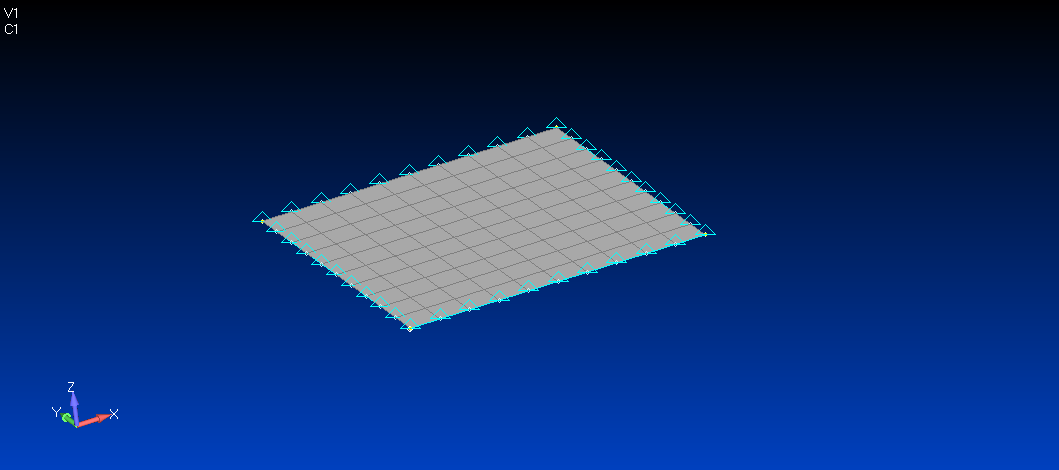
\includegraphics[scale=0.5]{figures/undef-model.png}
    \caption{FEM model.}
    \label{fig:model}
\end{figure}

The \emph{Vg} plot in Fig.\ref{fig:plot} indicates the flutter condition at mode 2 and mode 17 at 607 m/s and 741 m/s, respectively.

\begin{figure}[ht]
    \centering
    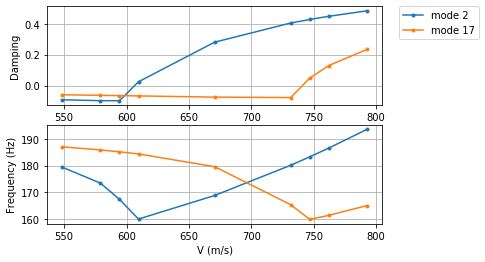
\includegraphics[scale=0.8]{figures/vfvg.png}
    \caption{Vg and Vf graphics for the critical modes 2 and 17.}
    \label{fig:plot}
\end{figure}

Using the Femap's interface is possible to visualize a animated model of most critical condition (mode 2 at 607 m/s), as indicated in Fig.\ref{fig:deform}.

\begin{figure}[ht]
    \centering
    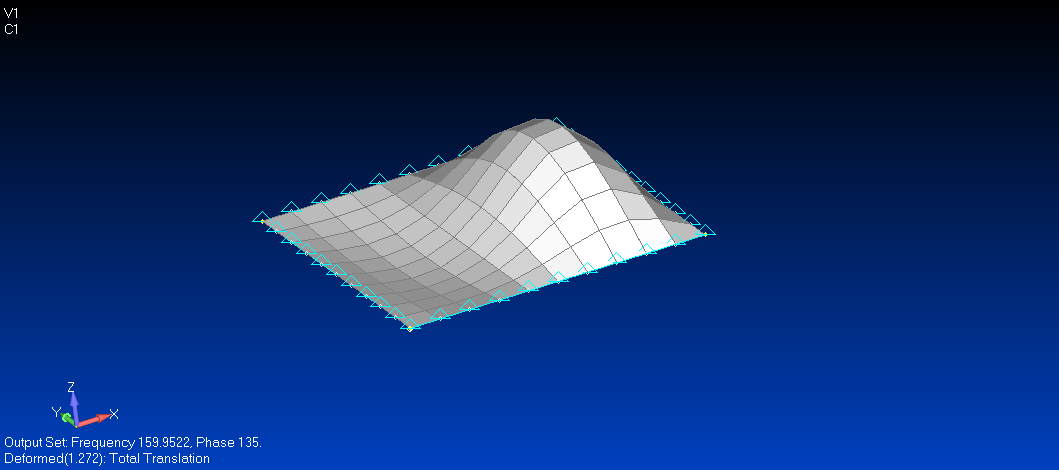
\includegraphics[scale=0.5]{figures/animated-model.png}
    \caption{Animated model view on Femap.}
    \label{fig:deform}
\end{figure}

% \begin{figure}[h!]
%     \centering
%     \includegraphics[scale=0.5]{figures/undef model.png}
%     \caption{FEM model.}
%     \label{fig:model}
% \end{figure}

% The expected results of the numerical analysis are a greater critical point of the stiffened configurations
% over the conventional configurations.
% %The boundary conditions and Mach number should have less influence in the critical point.
% The correlation of data with the literature is expected to be good, as the conditions applied
% on the numerical model are in the validity range of the linear model.

% The work of \citet{pacheco_finite_2018} has a analyzed a flat rectangular plate reinforced by a flexible beam.
% The results reached that ...